\documentclass{article}

% Language setting
\usepackage[spanish]{babel}
\usepackage{graphicx}
\graphicspath{{imagenes/}{evidencias/}}
\usepackage[colorlinks=true, allcolors=blue]{hyperref}
\usepackage[letterpaper,top=2cm,bottom=5cm,left=3cm,right=3cm,marginparwidth=1.75cm]{geometry}

% Useful packages
\usepackage{amsmath}
\usepackage{graphicx}
\usepackage[colorlinks=true, allcolors=blue]{hyperref}
\usepackage{amssymb}
\usepackage{fancyhdr}
\usepackage{lipsum}
\usepackage{multicol}
\usepackage{float}
\pagestyle{fancy}

\fancyhf{}
\setlength{\headheight}{70pt}

% Definición del encabezado
\fancyhead[C]{%
    \begin{minipage}[c]{1.5cm}
        \includegraphics[width=1.5cm]{imagenes/uta.png}
    \end{minipage}%
    \hfill
    \begin{minipage}[c]{10cm}
        \centering
        \small {\textbf{UNIVERSIDAD TÉCNICA DE AMBATO}} \\[0.1cm]
        \scriptsize \textit{FACULTAD DE INGENIERÍA EN SISTEMAS ELECTRÓNICA E INDUSTRIAL} \\[0.1cm]
        \scriptsize \textbf{CARRERA SOFTWARE} \\[0.1cm]
        \scriptsize \textbf{CICLO ACADÉMICO: ENERO - JULIO 2026}
        \vspace{0.2cm}
    \end{minipage}%
    \hfill
    \begin{minipage}[c]{1.5cm}
        \centering
        \includegraphics[width=1.5cm]{imagenes/fisei.png}
    \end{minipage}%
}

\begin{document}
\begin{center}
    {\large \textbf{INFORME DE GUÍA PRÁCTICA}} \\
\end{center}

\section{Portada}
\begin{flushleft}
\begin{tabular}{ l p{8cm} }
    \textbf{Tema:} & APE 5. Diseño de Interfaces Web Adaptables \\
    \textbf{Unidad de Organización Curricular:} & Profesional \\
    \textbf{Nivel y Paralelo:} & 5 - A \\
    \textbf{Alumnos participante(s):} & Velasco Huayamave Kevin Andrés \\& Miranda Tarupi Luis Sebastián \\ & García Amores Manolo José \\& Cholota Bastidas Ariel Isai \\
    \textbf{Asignatura:} & Interacción Humano/Computador \\
    \textbf{Docente:} & Ing. Caiza Caizabuano Jose Ruben \\
\end{tabular}
\end{flushleft}

\section{Informe de guía práctica}
\subsection{Objetivos}
\subsubsection{General}
Validar técnicamente una interfaz web adaptable del caso CaféU (confirmación de pedido), probarla con usuarios reales y defender las decisiones de diseño ante el grupo evaluador, consolidando la colaboración en GitHub.

\subsubsection{Específicos}
\begin{itemize}
    \item Implementar la versión adaptativa (Mobile-First) con HTML5 semántico, CSS y JavaScript.
    \item Verificar la ausencia de desborde horizontal en cuatro resoluciones (320, 360, 768 y 1366 px).
    \item Registrar la observación con usuarios en una tabla de pruebas.
    \item Responder las preguntas técnicas y la objeción de la defensa QA/UX.
    \item Consolidar las 4 ramas, los 4 Issues y los 4 Pull Requests en GitHub.
\end{itemize}

\subsection{Modalidad}
Presencial

\subsection{Tiempo de duración}
Presenciales: 2\\
No presenciales: 0

\subsection{Instrucciones}
\textbf{Acciones previas:}
\begin{itemize}
    \item Revisar el material de la asignatura sobre diseño de interfaces web adaptables.
    \item Tener la interfaz integrada (HTML, CSS y JavaScript) lista para probar.
    \item Preparar las capturas y las mediciones en las cuatro resoluciones.
\end{itemize}

\textbf{Pasos:}
\begin{enumerate}
    \item Probar la versión integrada en DevTools al 100 \% de zoom en 320, 360, 768 y 1366 px.
    \item Medir \texttt{scrollWidth} y comprobar que no supere \texttt{innerWidth}.
    \item Aplicar la consigna neutral a un compañero de otro grupo y registrar la observación.
    \item Responder la defensa cruzada QA/UX y registrar el acta.
    \item Cerrar los Issues mediante Pull Requests y elaborar el informe final.
\end{enumerate}

\subsection{Listado de equipos, materiales y recursos}
\textbf{Listado de equipos y materiales generales empleados en la guía práctica:}
\begin{itemize}
    \item Computadora
    \item Herramientas ofimáticas
    \item Aula virtual
    \item Internet
    \item Visual Studio Code y navegador con DevTools
\end{itemize}

\textbf{TAC (Tecnologías para el Aprendizaje y Conocimiento) empleados en la guía práctica:}
\begin{itemize}
    \item[$\square$] Plataformas educativas
    \item[$\square$] Simuladores y laboratorios virtuales
    \item[$\square$] Aplicaciones educativas
    \item[$\square$] Recursos audiovisuales
    \item[$\square$] Gamificación
    \item[$\blacksquare$] Inteligencia Artificial
    \item Otros (Especifique): \underline{\hspace{5cm}}
\end{itemize}

\subsection{Actividades por desarrollar}
\begin{enumerate}
    \item \textbf{Pruebas técnicas:} medir el desborde horizontal en cuatro resoluciones y documentar los resultados. \textbf{Producto:} \texttt{resultados/pruebas.md} y capturas en \texttt{evidencias/}.
    \item \textbf{Observación con usuarios:} aplicar una consigna neutral y registrar tiempo, errores, ayuda y dificultades. \textbf{Producto:} \texttt{resultados/checklist.md}.
    \item \textbf{Defensa QA/UX:} responder las dos preguntas técnicas y la objeción de diseño. \textbf{Producto:} \texttt{docs/preguntas.md}.
    \item \textbf{Cierre colaborativo:} consolidar las ramas, Issues y Pull Requests, y redactar las conclusiones. \textbf{Producto:} \texttt{docs/conclusiones.md} e informe final.
\end{enumerate}

\subsection{Resultados obtenidos}
El resultado de la práctica es una interfaz web adaptable de la confirmación de pedido de CaféU. En la Fase 1 se diagnosticó el desborde de la versión de escritorio y se definió la ficha de aplicación; en la Fase 2 se implementó la versión adaptativa, se validó en cuatro resoluciones y se defendió ante el grupo evaluador.

\subsubsection{Diagnóstico de la Fase 1 (Versión A)}
En la Fase 1 se identificó el problema del diseño inicial (Versión A): una pantalla de escritorio con un ancho fijo de 960 px. Al abrirse en un celular de 360 px, este ancho fijo produce dos consecuencias:

\begin{itemize}
    \item \textbf{Desborde horizontal:} el contenido no cabe en el viewport y aparece una barra de desplazamiento lateral.
    \item \textbf{Ocultamiento de información crítica:} el total a pagar y el botón ``Confirmar pedido'' quedan fuera de la vista, lo que obliga al usuario a hacer scroll para completar la acción.
\end{itemize}

\begin{figure}[H]
    \centering
    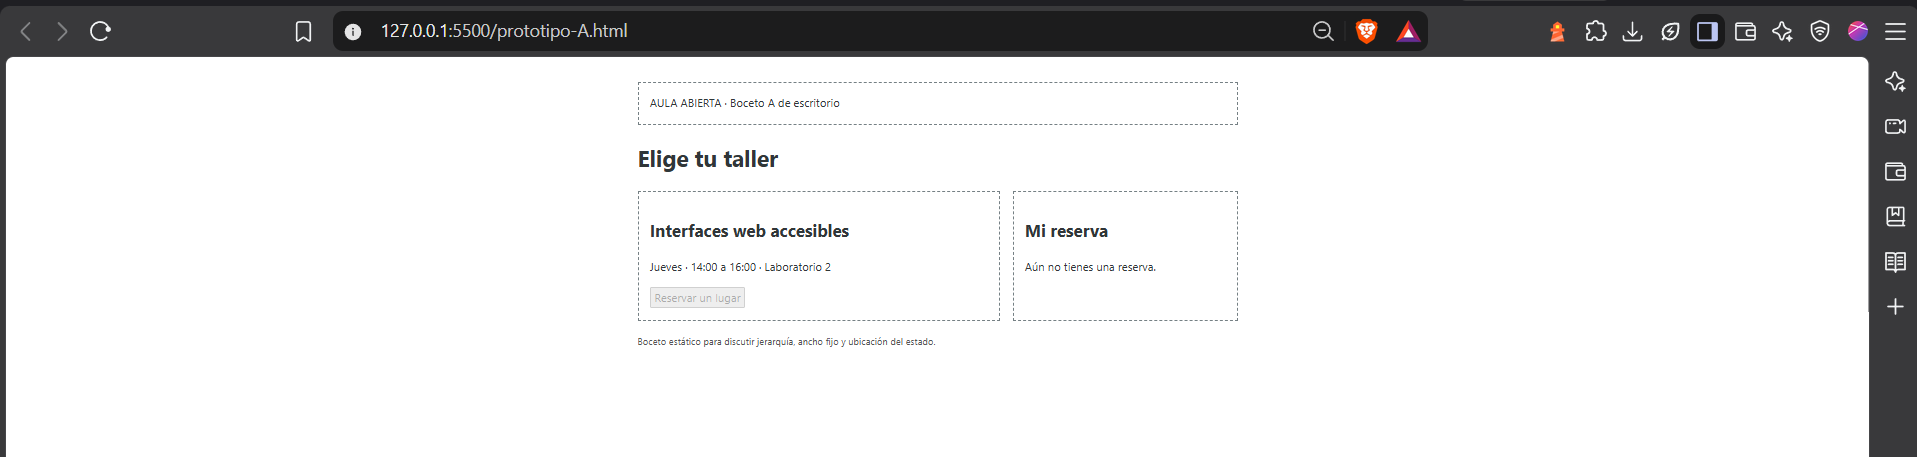
\includegraphics[width=0.45\textwidth]{imagenes/escritorio.png}
    \hfill
    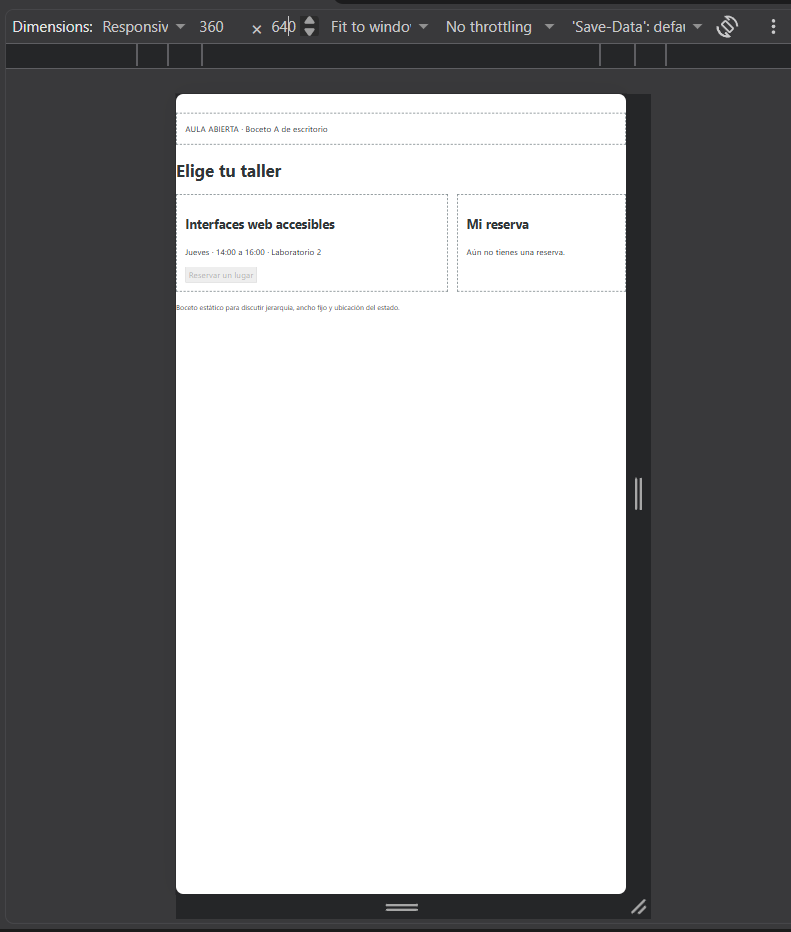
\includegraphics[width=0.45\textwidth]{imagenes/celular.png}
    \caption{Versión A de la Fase 1: escritorio (960 px) y celular con desborde.}
    \label{fig:fase1}
\end{figure}

\subsubsection{Ficha de aplicación}
\begin{center}
\begin{tabular}{|p{4.4cm}|p{9.0cm}|}
\hline
\textbf{Campo} & \textbf{Valor} \\
\hline
Actor & Estudiante universitario \\
\hline
Tarea principal & Confirmar un pedido (café y sánduche) \\
\hline
Dato clave que decide la acción & El total a pagar y el resumen de ítems \\
\hline
Acción principal & Botón ``Confirmar pedido'' \\
\hline
Resultado visible & Mensaje ``¡Pedido confirmado!'' con número \#CU-104 \\
\hline
Mecanismo para corregir o cancelar & Botón ``Cancelar pedido'' que revierte el estado \\
\hline
\end{tabular}
\end{center}

\subsubsection{Regla de interacción y criterio de aceptación}
\textbf{Regla de interacción:} impedir envíos duplicados. Al pulsar ``Confirmar pedido'', el botón se deshabilita (\texttt{disabled}) para que un segundo clic no genere un pedido duplicado.

\textbf{Criterio de aceptación medible:} tras el primer clic, el botón queda deshabilitado de inmediato y no se registra un segundo pedido aunque el usuario pulse repetidamente; el estado se anuncia con \texttt{role="status"}.

\subsubsection{Interfaz adaptativa (Versión B)}
Se implementó la pantalla ``Mi pedido'' y ``Confirmar pedido'' con tres archivos:
\begin{itemize}
    \item \texttt{src/index.html}: estructura HTML5 semántica con \texttt{<header>}, \texttt{<main>}, \texttt{<section>}, \texttt{<article>}, \texttt{<dl>} para los datos clave, botones nativos y \texttt{<p role="status">} para anunciar cambios de estado.
    \item \texttt{src/estilos.css}: enfoque Mobile-First estricto, una columna en móvil y dos columnas con \texttt{@media (min-width: 48rem)}, botones con \texttt{min-height: 44px} y foco visible con \texttt{:focus-visible}.
    \item \texttt{src/interaccion.js}: gestión de los tres momentos de la acción (Disponible $\rightarrow$ Confirmada $\rightarrow$ Cancelada), bloqueo de duplicados con \texttt{disabled} y gestión del foco con \texttt{.focus()}.
\end{itemize}

\subsubsection{Pruebas técnicas de desborde}
Se midió \texttt{document.documentElement.scrollWidth} en cuatro viewports y se verificó la ausencia total de desborde horizontal (\texttt{scrollWidth} $\leq$ \texttt{innerWidth}).

\begin{center}
\begin{tabular}{|c|c|c|c|}
\hline
\textbf{Viewport} & \textbf{innerWidth} & \textbf{scrollWidth} & \textbf{¿Desborde?} \\
\hline
320 $\times$ 720 & 320 & 320 & No \\
\hline
360 $\times$ 800 & 360 & 360 & No \\
\hline
768 $\times$ 1024 & 768 & 768 & No \\
\hline
1366 $\times$ 768 & 1366 & 1366 & No \\
\hline
\end{tabular}
\end{center}

\begin{figure}[H]
    \centering
    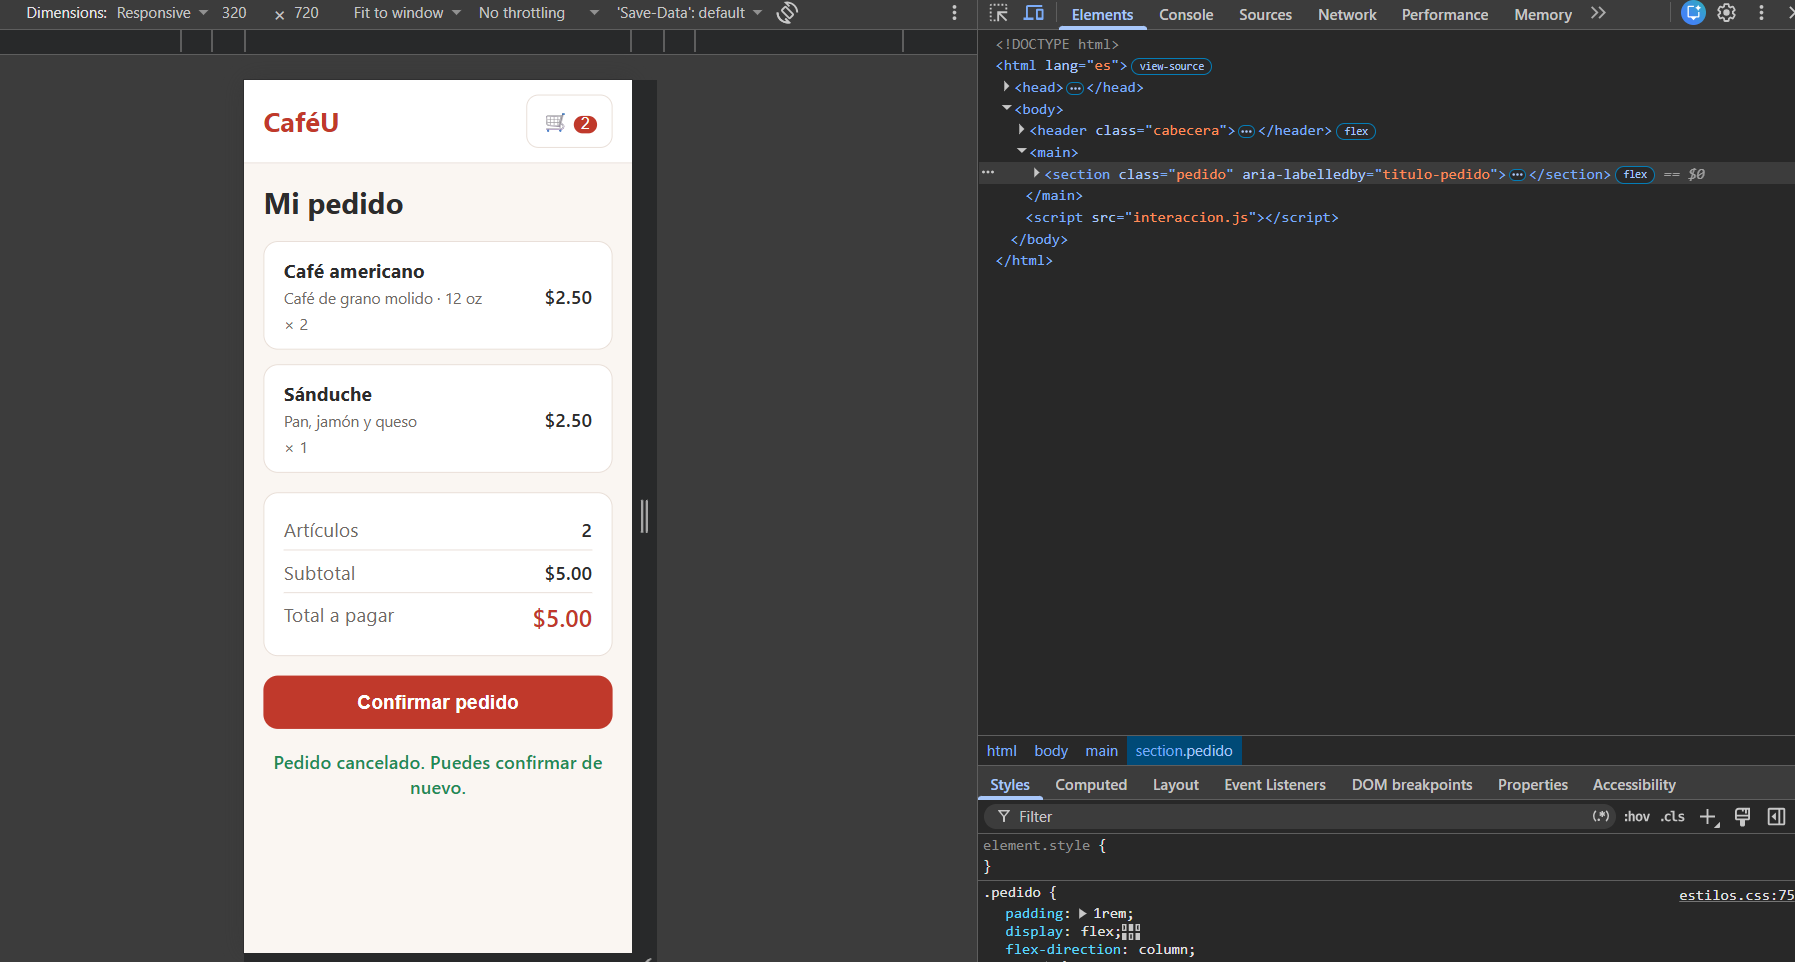
\includegraphics[width=0.99\textwidth]{imagenes/320x720.png}
    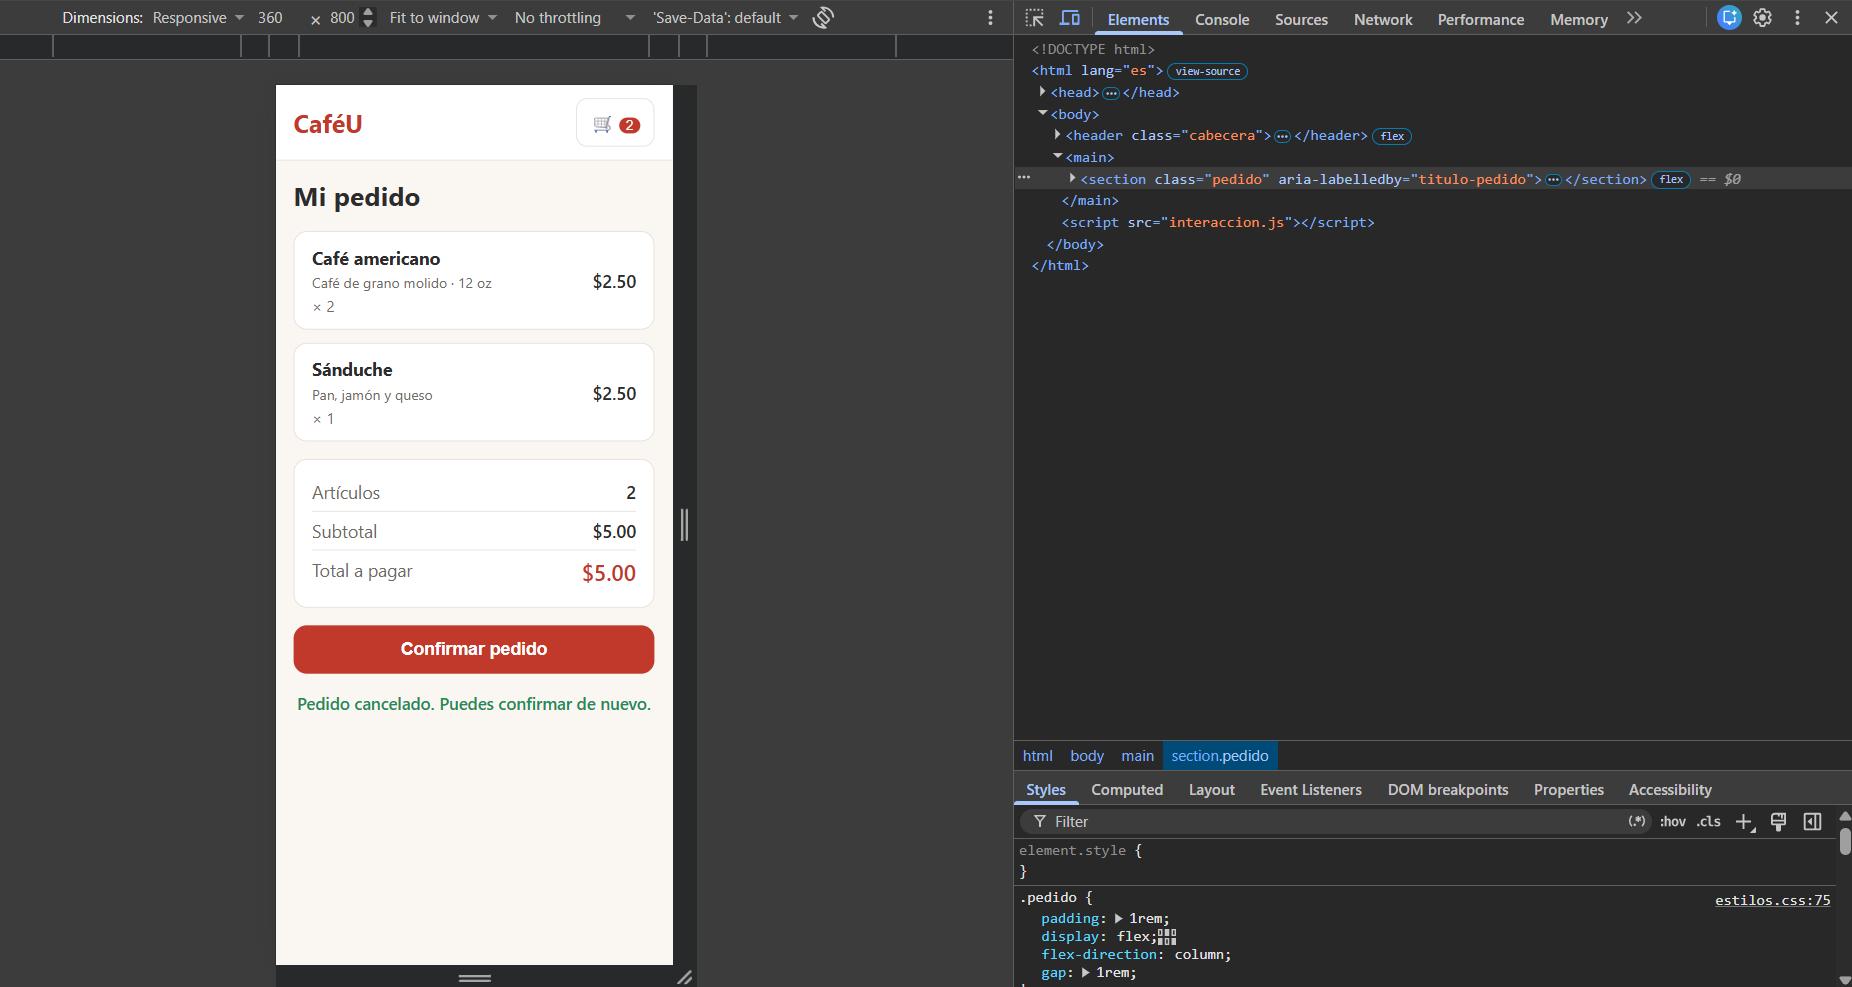
\includegraphics[width=0.99\textwidth]{imagenes/360x800.png}
    \caption{Validación en 320 $\times$ 720 y 360 $\times$ 800 px.}
    \label{fig:movil}
\end{figure}

\begin{figure}[H]
    \centering
    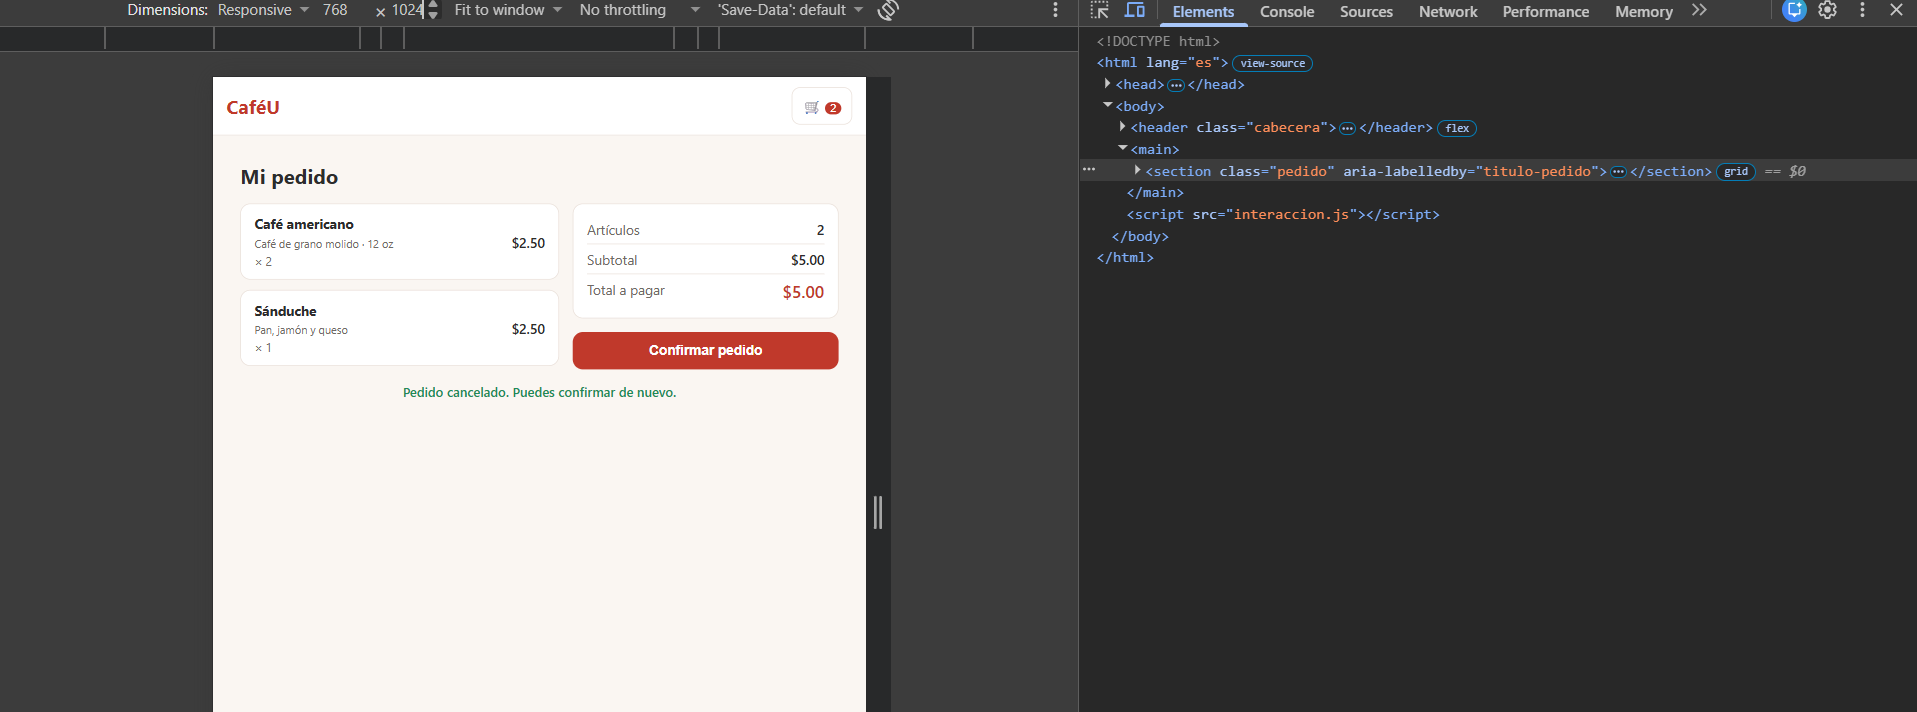
\includegraphics[width=0.99\textwidth]{imagenes/768x1024.png}
    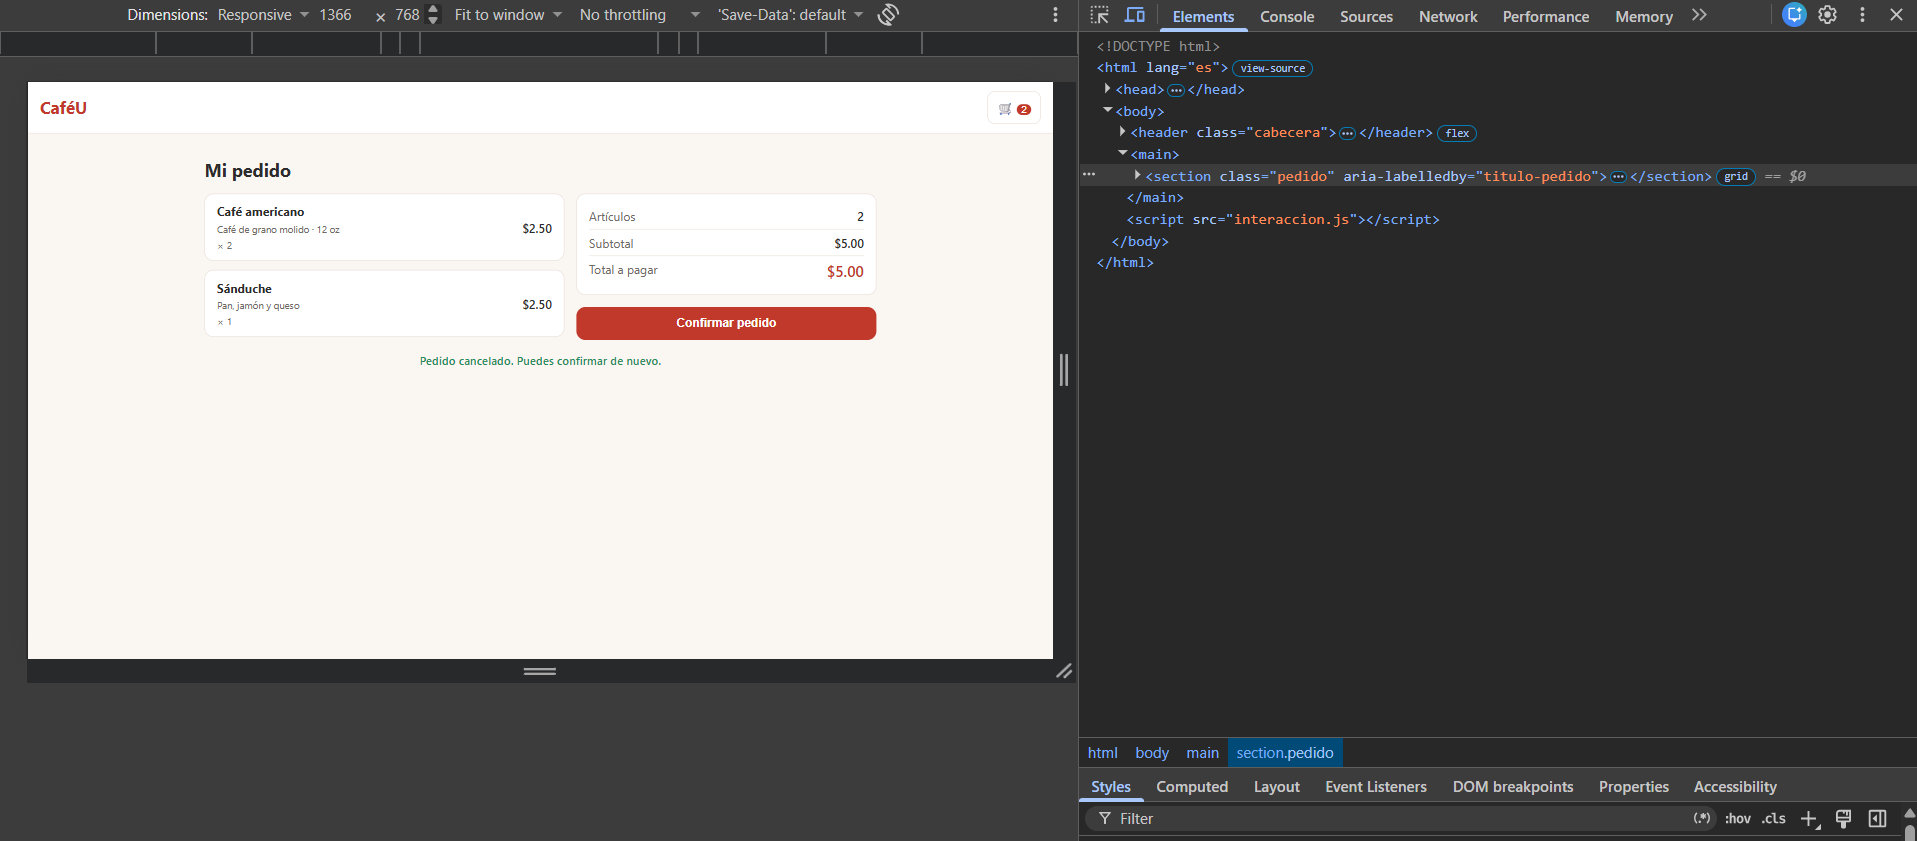
\includegraphics[width=0.99\textwidth]{imagenes/1366x768.png}
    \caption{Validación en 768 $\times$ 1024 y 1366 $\times$ 768 px.}
    \label{fig:escritorio}
\end{figure}

\subsubsection{Observación con usuarios}
Se aplicó una consigna neutral (``Confirma el pedido que aparece en pantalla'') a un compañero de otro grupo, sin indicar qué botones presionar.

\begin{center}
\begin{tabular}{|c|c|c|c|c|}
\hline
\textbf{Participante} & \textbf{Tiempo (s)} & \textbf{Errores} & \textbf{Ayuda} & \textbf{Dificultades} \\
\hline
Participante 1 (Grupo 3) & 18 & 0 & 0 & Ninguna \\
\hline
Participante 2 (Grupo 1) & 25 & 0 & 1 & Duda inicial sobre cuál botón confirma \\
\hline
\end{tabular}
\end{center}

\subsubsection{Defensa cruzada QA/UX}
Ante el grupo retador G3 se sustentaron dos preguntas técnicas y una objeción de diseño (el detalle completo está en \texttt{docs/preguntas.md}).

\textbf{Pregunta técnica 1} (punto de corte en CSS y orden con Tab). Al cruzar \texttt{48rem}, el contenedor cambia de una columna a dos mediante CSS Grid con \texttt{grid-template-areas}. El orden del DOM no cambia, por lo que la secuencia de tabulación sigue el orden del documento y es idéntica en móvil y escritorio.

\textbf{Pregunta técnica 2} (prevención de envíos duplicados y foco). Al confirmar se ejecuta \texttt{btnConfirmar.disabled = true}, se anuncia el resultado con \texttt{role="status"} y el foco se traslada con \texttt{btnCancelar.focus()}. Al cancelar, se restaura el botón y el foco vuelve a ``Confirmar pedido''.

\textbf{Objeción de diseño} (ajuste geométrico frente a comprensión). El CSS resuelve que la interfaz quepa (ajuste geométrico); la comprensión se logra con semántica HTML, etiquetas claras, mensajes de estado y foco visible. Ambas evidencias se entregan juntas.

\subsubsection{Entregables en GitHub}
\begin{enumerate}
    \item Código adaptativo en \texttt{src/} (HTML, CSS, JavaScript).
    \item Resultados de pruebas en \texttt{resultados/} y capturas en \texttt{evidencias/}.
    \item Defensa y conclusiones en \texttt{docs/}.
    \item 4 ramas integradas en \texttt{main}, 4 Issues cerrados y 4 Pull Requests revisados.
    \item Enlace al repositorio: \url{https://github.com/Sax300-cpu/HCI-2026-G2}
\end{enumerate}

\subsection{Habilidades blandas empleadas en la práctica}
\begin{itemize}
    \item[$\blacksquare$] Liderazgo
    \item[$\blacksquare$] Trabajo en equipo
    \item[$\square$] Comunicación asertiva
    \item[$\square$] La empatía
    \item[$\blacksquare$] Pensamiento crítico
    \item[$\square$] Flexibilidad
    \item[$\square$] La resolución de conflictos
    \item[$\square$] Adaptabilidad
    \item[$\blacksquare$] Responsabilidad
\end{itemize}

\subsection{Conclusiones}
\begin{itemize}
    \item La interfaz adaptativa de CaféU no genera desborde horizontal en las cuatro resoluciones, lo que confirma la efectividad del enfoque Mobile-First y del punto de corte en 48rem.
    \item El bloqueo del botón con \texttt{disabled} y la gestión explícita del foco evitan envíos duplicados y mantienen al usuario ubicado.
    \item La validación combinada (mediciones técnicas y observación con usuarios) demuestra tanto el ajuste visual como la comprensión del estado.
\end{itemize}

\subsection{Recomendaciones}
\begin{itemize}
    \item Probar la interfaz en distintos navegadores y con lectores de pantalla reales.
    \item Ampliar la muestra de participantes para obtener mediciones más representativas.
    \item Persistir el estado del pedido (pendiente/confirmado) para evitar pérdida de datos al recargar.
\end{itemize}

\subsection{Referencias}
\begin{itemize}
    \item ISO. (2019). \textit{ISO 9241-210:2019 Ergonomics of human-system interaction — Part 210: Human-centred design for interactive systems}. \href{https://www.iso.org/standard/77520.html}{iso.org/standard/77520.html}
    \item Nielsen, J. (1994). \textit{10 Usability Heuristics for User Interface Design}. Nielsen Norman Group. \href{https://www.nngroup.com/articles/ten-usability-heuristics/}{nngroup.com}
    \item W3C. (2023). \textit{Web Content Accessibility Guidelines (WCAG) 2.2}. \href{https://www.w3.org/TR/WCAG22/}{w3.org}
    \item MDN Web Docs. \textit{Responsive design}. \href{https://developer.mozilla.org/en-US/docs/Learn/CSS/CSS_layout/Responsive_Design}{developer.mozilla.org}
\end{itemize}

\vspace{-3em}
% \renewcommand{\refname}{}
% \bibliographystyle{ieeetr}
% \bibliography{sample}

\end{document}
